% Ella-Lovise  is writing

\subsection*{Problem 2.4}
\addcontentsline{toc}{subsection}{Problem 2.4}

\subsubsection*{Calculate sideslip angle}
\addcontentsline{toc}{subsubsection}{Calculate sideslip angle}

The sideslip angle is as the angle from $x_b$ axis of {b} to the velocity vector of the vehicle,positive rotation about the $z_b$ axis of {b} by the right-hand screw convetion. The formmula forsideslip is therfore:
\begin{equation}
    \boldsymbol{\beta}_r = \arcsin( v_r/U_r)
    \label{eq:beta_r}
\end{equation}
defined by the relative velocity $v_r$ and relative speed $U_r$. The relative velocity defined as \eqref{eq:v_r}. To find the relative velocity is it needed to rotate either the velocity of the vechicle or current. The relative velocity of the vehicle in ned-referance frame is:

\begin{equation}
    \boldsymbol{v}^b_r = \boldsymbol{v}^b_{b/c} - \boldsymbol{v}^{b}_{c/n} =  \boldsymbol{v}^b_{b/c} - \mathbf{R}^b_n \boldsymbol{v}^{n}_{c/n} 
    \label{eq:v_b_r}
\end{equation}

The crab angle for the vehicle moving in the straight line was found by first calculating the realtive velocity , using equation \eqref{eq:v_b_r}, with  the velocity of  on a straight line  $\mathbf{v}_b^b = [1.5, 0, 0]$, found in assignemnt 2.1, and   the current velocity was calculated in assignment 2.3, using equation \eqref{eq:v_n_c}. \todo{Should i say something about the approximation}. The crab angle was calculated using equation \eqref{eq:beta_r}, giving sideslip angle of $7.2084 ^\circ$. \todo{check if Alexandra agree} This means the vehicle is moving upwards relative to current, relative to body-frame. This makes  Since the vehicle and the current are moving in different directions, the sideslip angle is negative. \todo{ CONFUSED, ASK ALEXANDRA!}

\subsubsection{Simulation of translational motion of the vehicle on the circle}

The simulation of the translational motion was done by simulation in \texttt{MATLAB}. To simulate the translational motion without current, first the velocity of the vehicle was calculated :
\begin{equation}
    \mathbf{v}^n_{b/c} = \mathbf{R}^n_b \mathbf{v}^b_{b/c} = \mathbf{R}^n_b [U*cos(\omega t), U*sin(\omega t), 0]^\top
    \label{eq:v_n_b_c}
\end{equation}


 The position of the vechicle was found by using euler integration,meaning the position in ned for vecickle $\mathbf{p}(i+1)^n_b = \mathbf{p}(i)^n_b + \mathbf{v}(i)^n_b*h $, with $h = 0.1$, which is the simulation step.
 
The  simulation of  the translational motion with current, was choosen to be simulated realtive to ned-referanceframe with the position relative to the ocean-surface, and not relative to the current. \todo{Agree Alexandra? Jeg forstår ikke helt hva setningen sier..?}. The first step was to calculated the velocity of the vehicle $\mathbf{v}^n_{b/c}$, as done in \eqref{eq:v_n_b_c}. Further the velocity of the current realtive to ned, expressed in ned $\mathbf{v}^n_{c/n}$ was calculated, from equation \eqref{eq:v_n_c}. The expression for the velocity of the vehicle relative to ned-referanceframe and relative to the ocean-surface ( meaning boat is moving with current) is:

\begin{equation}
    \mathbf{v}^n_{b/n} = \mathbf{v}^n_{b/c} + \mathbf{v}^n_{c/n}
\end{equation}

The expression for the position of the vechicle relative to ned-referanceframe and relative to the ocean-surface is found by euler integration, meaning $\mathbf{p}(i+1)^n_b = \mathbf{p}(i)^n_b + \mathbf{v}(i)^n_b*h $, with $h = 0.1$. Same method as for the simulation without current.

The velocity of vehicle relative to the boat with current is calculated by using:

\begin{equation}
    \mathbf{v}^n_{b/n} = \mathbf{v}^n_{b/c} - \mathbf{v}^n_{c/n}
\end{equation}.

The plots after the simulation are:




\subsection*{Problem 2.5}

The Nomoto model can be written as
\begin{equation}
	\frac{r}{\delta} (s) = \frac{K}{Ts+1}
\end{equation}
and the equations for the roll and pitch rate as
\begin{equation}
\begin{aligned}
	&\dot{p} + 2\zeta_p\omega_p p + \omega_p^2 \phi = 0\\
	&\dot{q} + 2\zeta_q\omega_q q + \omega_q^2 \theta = 0
\end{aligned}
\end{equation}

\subsection*{Problem 2.6}
References can be placed in the bibliography.bib and referred to as \cite{Fossen2011} and \cite{Fjellstad1994857}.


% files added by teacher

Answer Problem 2.4 here. Figures can be inserted as:
\begin{figure}[ht]
	\centering
	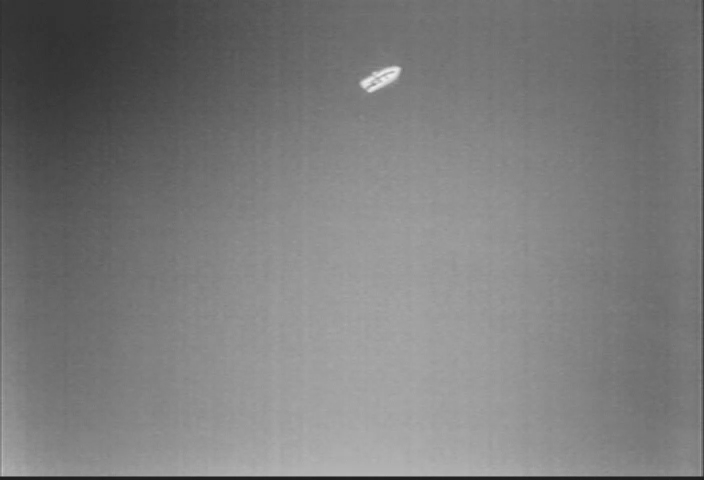
\includegraphics[width=0.7\textwidth]{assignment_1/rapport/figures/fig1} 
	\caption{Figure of something useful.}
	\label{fig:fig1}
\end{figure}

You can now refer to this figure as \figref{fig:fig1}. You can also insert figures side-by-side:
\begin{figure}[ht]
	\centering
	\begin{subfigure}[b]{0.45\textwidth}
		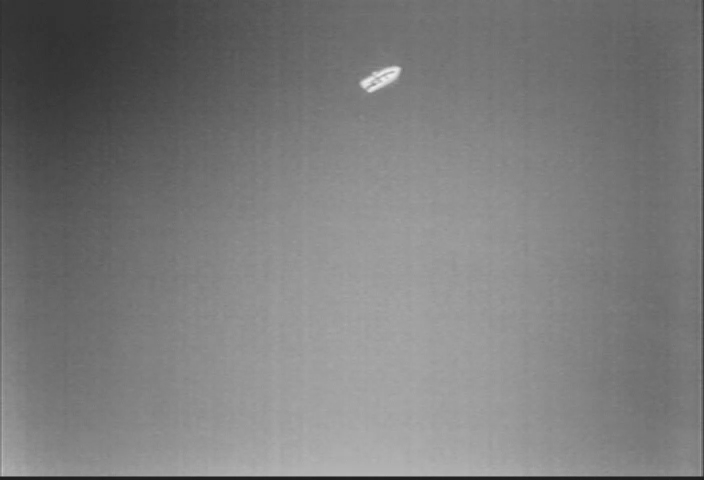
\includegraphics[width=\textwidth]{assignment_1/rapport/figures/fig1}
		\caption{caption..}
		\label{fig:2a}
	\end{subfigure}
	~ %add desired spacing between images, e. g. ~, \quad, \qquad, \hfill etc. 
	%(or a blank line to force the subfigure onto a new line)
	\begin{subfigure}[b]{0.45\textwidth}
		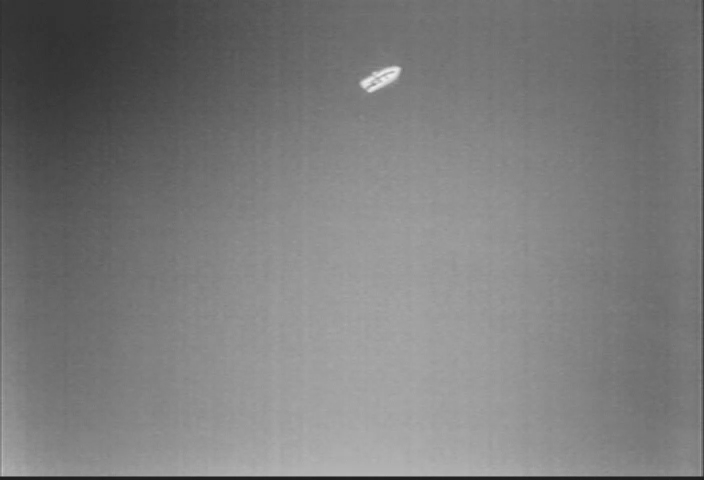
\includegraphics[width=\textwidth]{assignment_1/rapport/figures/fig1}
		\caption{caption..}
		\label{fig:2b}
	\end{subfigure}
	\begin{subfigure}[b]{0.45\textwidth}
		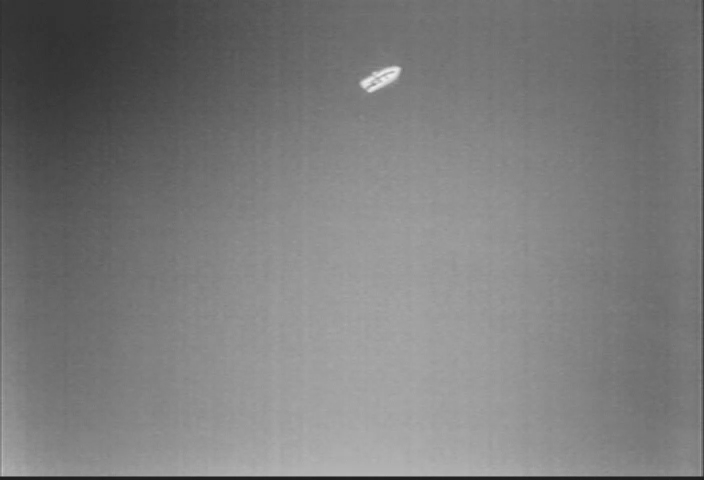
\includegraphics[width=\textwidth]{assignment_1/rapport/figures/fig1}
		\caption{caption..}
		\label{fig:2c}
	\end{subfigure}
	\begin{subfigure}[b]{0.45\textwidth}
		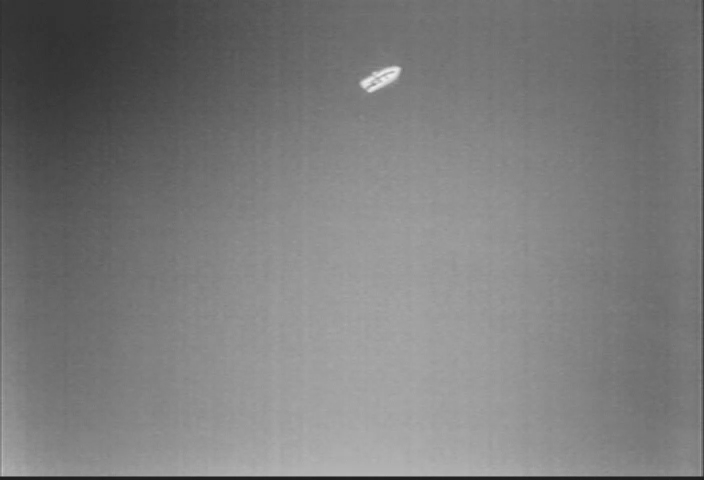
\includegraphics[width=\textwidth]{assignment_1/rapport/figures/fig1}
		\caption{caption..}
		\label{fig:2d}
	\end{subfigure}		
	\caption{Caption for all figures}\label{fig:2}
\end{figure}